\documentclass[11pt,a4paper]{scrartcl}
\typearea{12}
\usepackage{graphicx}
\usepackage{pstricks}
\usepackage{listings}
\usepackage{tikz-qtree}
\lstset{language=C}
\pagestyle{headings}
\markright{COMS11600 - Principles of programming IV.3}
\begin{document}
\tikzset{every tree node/.style={minimum width=2em,draw,circle},
         blank/.style={draw=none},
         edge from parent/.style=
         {draw,->, edge from parent path={(\tikzparentnode) -- (\tikzchildnode)}},
         level distance=1.5cm}

\subsection*{IV.2 Data structures - AVL trees}

An AVL tree is a balanced binary search tree; because it is balanced
binary search is a $O(\log{n})$ operation. It is named for
G. M. Adelson-Velskii and E. M. Landis who invented it in 1962. AVL
trees augment ordinary binary trees in two ways, first: every node has
an extra piece of information called the balance factor and second:
there are algorithms, called rotations, to rearrange the tree so that
it is still a binary search tree but one where every node has a
balance factor of one, zero or -1, corresponding to near perfect
balance. The new node definition is given in Table~\ref{c_node} and
the new constructor is given in Table~\ref{c_make}.

\begin{table}[b]
\begin{lstlisting}[numbers=left]
struct node
{
  int entry;
  int balance;
  struct node *left;
  struct node *right;
};
\end{lstlisting}
\caption{A node, it has a variable to store the entry and pointers to
  the left and right children. It also has a new int to keep track of
  how balanced the node is.\label{c_node}}
\end{table}


\begin{table}
\begin{lstlisting}[numbers=left]

struct node * make_node(int new_entry)
{
  struct node * a_node=(struct node *)malloc(sizeof(struct node));
  a_node->entry=new_entry;
  a_node->balance=0;

  return a_node;
}
\end{lstlisting}
\caption{Making a node, the new thing is that the balance is initialized to zero.\label{c_make}}
\end{table}



The {\sl height} of a tree is the maximum number of nodes from the
root to a leaf travelling down the pointers. This is illustrated in
Fig.~\ref{fig_example_tree}. The {\sl balance} of a node is a measure
of the difference in height of the two subtrees the node has, the left
subtree and the right subtree. Specifically, if height({\bf a\_node}) gives the
height of a node called {\bf a\_node} then
\begin{equation}
\mbox{{\bf a\_node}}->\mbox{balance}=\mbox{height}(\mbox{{\bf
    a\_node}}->\mbox{left})-\mbox{height}(\mbox{{\bf
    a\_node}}->\mbox{right})
\end{equation}
In practise the balance factors will be updated as nodes are added,
rather than calculated by explicitly computing heights; this will be
looked at later, for now all that's important is that the balance is
the difference in heights. A tree with the balance factors written in
is given in Fig.~\ref{fig_example_balance}. A tree is called {\sl
  balanced} if all the balance factors are one, zero or -1; this makes
sense since it is impossible to have a tree with all nodes having
balance zero unless the number of nodes is $2^r-1$, for some $r$. It
should be remembered that the height is what is important for binary
search and you can see from Fig.~\ref{fig_odd_balance} that balanced
trees don't always have the same number of nodes on each side.

\begin{figure}
\begin{center}
\begin{tikzpicture}
\Tree [.50 [.20 \edge[]; {10} \edge[]; {25} ] [.70 \edge[blank];
    \node[blank]{}; \edge[]; [.80 \edge[]; {75} \edge[]; {95} ] ] ]
\end{tikzpicture}
\end{center}
\caption{An example binary tree for looking at heights. The node 50
  has height four, the distance down to 75 and 95. The node 20 has height two
  and the node 70 has height three.\label{fig_example_tree}}
\end{figure}

\begin{figure}
\begin{center}
\begin{tikzpicture}
\Tree
[.1     
    [.0 
      \edge[]; {0}
      \edge[]; {0}
    ]
    [.-2  
    \edge[blank]; \node[blank]{};
    \edge[]; [.1
                \edge[]; {0}
                \edge[blank]; \node[blank]{};
              ]
    ]
]
\end{tikzpicture}
\end{center}
\caption{An example binary tree with the balance factors shown.\label{fig_example_balance}}
\end{figure}


\begin{figure}
\begin{center}
\begin{tikzpicture}
\Tree
[.1     
    [.-1 
      \edge[]; {0}
           [.0
             \edge[]; {0}
             \edge[]; {0}
           ]
    ]
    [.-1  
    \edge[blank]; \node[blank]{};
    \edge[]; {0}
    ]
]
\end{tikzpicture}
\end{center}
\caption{An example of a balanced tree that may not look very balanced. The numbers are the balance factors.\label{fig_odd_balance}}
\end{figure}

Now, imagine adding a node causes one of its ancestors to have a
balance factor of two or minus two. If the tree was balanced before
the new node was added this is the worst case: adding a node changes
balance factors by one or minus one at the most. Now to fix the lack
of balance a rotation is used. There are actually four different
rotations corresponding to four classes of cases, all cases fall into
one of the four classes. We will examine two rotations here, it will
then be clear the remaining two rotations are mirror images. 

The two cases we look at are ones where the ancestor, which we will
call {\bf here}, has balance +2 and the two different rotations
correspond to 
\begin{equation}
\mbox{{\bf here}}->\mbox{left}->\mbox{balance}=1 
\end{equation}
and 
\begin{equation}
\mbox{{\bf here}}->\mbox{left}->\mbox{balance}=-1 
\end{equation}
In the first case the disbalance is on the left of the left subtree of
{\bf here}. This is the left-left case and the corresponding rotation is
called a left-left, or LL, rotation. In the second case it is on the
right of the left subtree of here and the corresponding rotation is
called a left-right, or LR, rotation. As a notational aside, the LL
rotation is sometimes just called the left rotation since it looks more
like a single rotation whereas the LR rotation looks like a double
rotation.

Lets examine the LL rotation first. The tree at Fig.~\ref{fig_LL} is
in need of such a rotation. The node {\bf here}$->$left is called {\bf
  left}. The first step is to remove the subtree rooted in {\bf left}
from {\bf here} and attach {\bf left}$->$right in its place. This is
shown in Fig.\ref{fig_LL_1}. Next, the subtree rooted in {\bf here} is
attached as the right subtree of {\bf left}. The pointer to {\bf here}
would then be updated to point to {\bf left}, the new root. This is
shown in Fig.~\ref{fig_LL_2}. 

The same set of instructions would have applied in the simpler looking
case Fig.~\ref{fig_LL_simple}, the only difference is that some of the
pointers in this case are NULL rather than pointing to nodes. The
rotation would also fix the more complicated case
Fig.~\ref{fig_LL_complicated} in which some of the nodes in the case
we looked at have been replaced by subtrees. Again the same instructions in
terms of pointers to nodes and where they get moved to will work. Code
to do the LL rotation is given in Table~\ref{c_LL}.

\begin{figure}
\begin{center}
\begin{tikzpicture}
\Tree
[.20:2     
  [.10:1
    [.5:1
      \edge[]; {1:0}
      \edge[blank]; \node[blank]{};
    ]
    \edge[]; {15:0}
  ]
  \edge[]; {30:0}
]
\end{tikzpicture}
\end{center}
\caption{A tree in need of a LL rotation. Example data values are
  given before the colon, the balance factor after. The 20 node is the
  ancestor, called {\bf here} in the text and the 1 node is the new
  node, the one that has just been added.\label{fig_LL}}
\end{figure}

\begin{figure}
\begin{center}
\begin{tikzpicture}
  \Tree
      [.10
        [.5
          \edge[]; {1}
          \edge[blank]; \node[blank]{};
        ]
        \edge[blank]; \node[blank]{};
      ]
\end{tikzpicture}
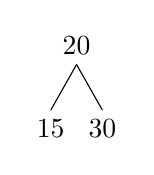
\begin{tikzpicture}
  \Tree
      [.20     
        \edge[]; {15}
        \edge[]; {30}
      ]
\end{tikzpicture}
\end{center}
\caption{LL step 1. The left subtree has been snapped off and replaced by what
  was the right subtree of {\bf left}.\label{fig_LL_1}}
\end{figure}

\begin{figure}
\begin{center}
\begin{tikzpicture}
\Tree
[.10:0
  [.5:1
    \edge[];{1:0}
    \edge[blank];\node[blank]{};
  ]
  [.20:0     
    \edge[]; {15:0}
    \edge[]; {30:0}
  ]
]
\end{tikzpicture}
\end{center}
\caption{LL step 2. The {\bf here} subtree has been attached as the
  right subtree of {\bf left}. The updated balance factors are given
  after the colons.\label{fig_LL_2}}
\end{figure}


\begin{figure}
{\bf A}
\begin{center}
\begin{tikzpicture}
  \Tree
      [.10:2
        [.5:1
          \edge[]; {1:0}
          \edge[blank]; \node[blank]{};
        ]
        \edge[blank]; \node[blank]{};
      ]
\end{tikzpicture}
\end{center}
{\bf B}
\begin{center}
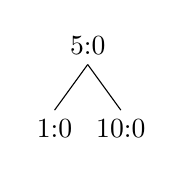
\begin{tikzpicture}
  \Tree
      [.5:0     
        \edge[]; {1:0}
        \edge[]; {10:0}
      ]
\end{tikzpicture}
\end{center}
\caption{Another LL rotation. {\bf A} represents before and {\bf B}
  after. Here the 5 node has no right node, so the right pointer of 10
  remains set to NULL, but following the same instructions gives the rotation.\label{fig_LL_simple}}
\end{figure}

\begin{figure}
{\bf A}
\begin{center}
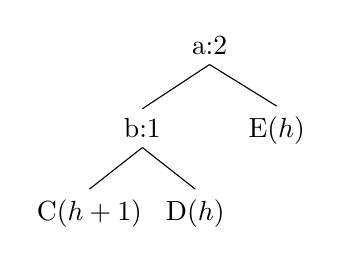
\begin{tikzpicture}
\Tree
[.a:2     
  [.b:1
    \edge[]; \node[very thick,rectangle]{C($h+1$)};
    \edge[]; \node[very thick,rectangle]{D($h$)};
  ]
  \edge[]; \node[very thick,rectangle]{E($h$)};
]
\end{tikzpicture}
\end{center}
{\bf B}
\begin{center}
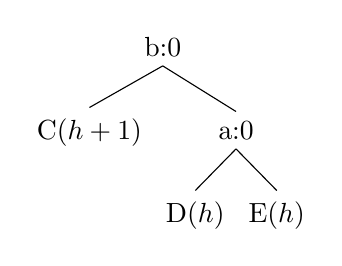
\begin{tikzpicture}
\Tree
[.b:0     
  \edge[]; \node[very thick,rectangle]{C($h+1$)};
  [.a:0
    \edge[]; \node[very thick,rectangle]{D($h$)};
    \edge[]; \node[very thick,rectangle]{E($h$)};
  ]
]
\end{tikzpicture}
\end{center}
\caption{{\bf A}: A tree in need of a LL rotation. Circles correspond
  to node and rectangles to whole subtrees, the number in brackets in
  the rectangles gives the height of the corresponding subtree, $h$ is
  some integer. The subtree at C is has height one greater than the
  subtree at D and the whole subtree rooted in B is has height two
  greater than the subtree at E. {\bf B} shows the same tree after the
  LL rotation.\label{fig_LL_complicated}}
\end{figure}


\begin{table}
\begin{lstlisting}[numbers=left]
struct node * rotate_ll(struct node * here)
{
  struct node * left = here->left;
  here->left=left->right;
  left->right=here;
  here->balance=0;
  here=left;
  here->balance=0;

  return here;
}
\end{lstlisting}
\caption{The LL rotation. In line 3 a new pointer is made to keep
  track of {\bf here}$->$left. This is now snapped off and {\bf
    here}$->$left set to point at {\bf left}$->$right instead in line 4,
  {\bf left}$->$right is then set pointing to {\bf here} in line 5. {\bf
    left} is now the root, so in line 7 the {\bf here} pointer is set
  to {\bf left}.\label{c_LL}}
\end{table}

Now, we consider the LR case. The tree at Fig.~\ref{fig_LR} is in need
of a LR rotation. Again, the disbalanced ancestor is called {\bf here}
and the left node of this ancestor is called {\bf left}. It turns out
we also need to keep track of {\bf left}$->$right and this node is
called {\bf left\_right}. The new node has been added to {\bf
  left\_right}, the new node could be the left or the right node of
{\bf left\_right}, in the figure both possibilities are shown, the
left dashed and the right dotted, only one of these two will happen at
one time.

\begin{figure}
\begin{center}
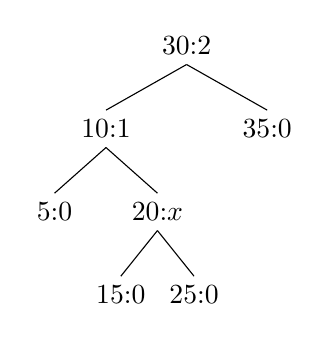
\begin{tikzpicture}
\Tree
[.30:2
  [.10:1
    \edge[]; {5:0}
         [.20:$x$
           \edge[]; \node[dashed]{15:0};
           \edge[]; \node[dotted]{25:0};
         ]
  ]
  \edge[]; {35:0}
]
\end{tikzpicture}
\end{center}
\caption{A tree in need of a LR rotation. The 30 node is the one
  called {\bf here}, the 10 node is {\bf left} and the 20 node is {\bf
    left\_right}. The new node is 15 or 25, the 15 is shown dashed and
  the 25 dotted since only one of 15 and 25 can be present, the other
  is NULL. The balance of 20 depends on which case we are dealing
  with, for the case where the new node is 15, the dashed case, $x=1$,
  for the dotted case, $x=-1$.\label{fig_LR}}
\end{figure}

Now, {\bf left\_right} is snapped off. One of its two nodes is the new
node. If it is the left node this is attached at the right of {\bf
  left}, where {\bf left\_right} used to be, that is the case
illustrated in the figure as the dashed case in
Fig.~\ref{fig_LR_1}. Next, the subtree rooted in {\bf left} is snapped
off and attached at the right of {\bf left\_right}. If the new node
was to the right of {\bf left\_right} this is attached to the left of
{\bf here}. This is the dotted case in the figure, which for step 2 is
Fig.~\ref{fig_LR_2}. Finally, the subtree rooted in {\bf here} is
attached to the right of {\bf left\_right} and the pointer that
pointed to here is set pointing to {\bf left\_right}. This is shown in
Fig.~\ref{fig_LR_3}.

\begin{figure}
\begin{center}
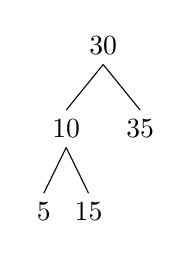
\begin{tikzpicture}
\Tree
[.30
  [.10
    \edge[]; {5}
    \edge[]; \node[dashed]{15};
  ]
  \edge[];{35}
]
\end{tikzpicture}
\begin{tikzpicture}
\Tree
[.20
           \edge[blank]; \node[blank]{};
           \edge[]; \node[dotted]{25};
]
\end{tikzpicture}
\end{center}
\caption{The first step of LR rotation. The 20 node is {\bf
    left\_right}, it has been snapped off the tree. If the new node is
  the 15 node it takes the place of the {\bf left\_right} node on the
  right of {\bf left}.  If the new node is the 25 node, that is
  attached on the left of {\bf here}.\label{fig_LR_1}}
\end{figure}


\begin{figure}
\begin{center}
\begin{tikzpicture}
\Tree
[.20
  [.10
    \edge[]; {5}
    \edge[]; \node[dashed]{15};
  ]
           \edge[blank]; \node[blank]{};
]
\end{tikzpicture}
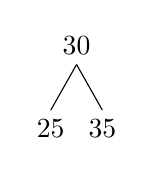
\begin{tikzpicture}
\Tree
[.30
  \edge[]; \node[dotted]{25};
  \edge[];{35}
]
\end{tikzpicture}
\end{center}
\caption{The second step of LR rotation. The 10 node, which is called {\bf left} has been snapped off the tree and attached to the left of {\bf left\_right} instead. \label{fig_LR_2}}
\end{figure}


\begin{figure}
\begin{center}
\begin{tikzpicture}
\Tree
[.20:0
  [.10:$y$
    \edge[]; {5:0}
    \edge[]; \node[dashed]{15:0};
  ]
  [.30:$z$
    \edge[]; \node[dotted]{25:0};
    \edge[blank]; \node[blank]{};
    \edge[];{35:0}
]
]
\end{tikzpicture}
\end{center}
\caption{The third step of LR rotation. {\bf here} is attached to the
  right of {\bf left\_right} and balance is restored. The balance
  factors $y$ and $z$ depend on whether this is the dotted or dashed
  case, for dashed $y=0$ and $z=-1$ and for dotted $y=1$ and
  $z=0$.\label{fig_LR_3}}
\end{figure}

As with the LL rotation, the example we looked at is standing in for a
whole class of exampled. Of course, for the LR rotation we actually
looked at two examples at once, the dotted example and the dashed
example, but there is a simpler case, given in
Fig.~\ref{fig_LR_simple} where some of the nodes are replaced with
NULLs, but, more importantly, there is a more general case where some
of the nodes are replaced by subtrees; this is given in
Fig.~\ref{fig_LR_complicated}.


\begin{figure}
{\bf A}
\begin{center}
\begin{tikzpicture}
  \Tree
      [.30:2
        [.10:-1
          \edge[blank]; \node[blank]{};
          \edge[]; {20:0}
        ]
        \edge[blank]; \node[blank]{};
      ]
\end{tikzpicture}
\end{center}
{\bf B}
\begin{center}
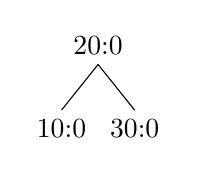
\begin{tikzpicture}
  \Tree
      [.20:0     
        \edge[]; {10:0}
        \edge[]; {30:0}
      ]
\end{tikzpicture}
\end{center}
\caption{Another LR rotation. {\bf A} represents before and {\bf B}
  after. Here {\bf left\_right} is also a leaf, but following the same
  instructions gives the rotation.\label{fig_LR_simple}}
\end{figure}



\begin{figure}
{\bf A}
\begin{center}
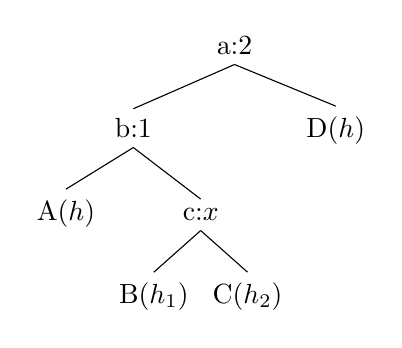
\begin{tikzpicture}
\Tree
    [.a:2
      [.b:1
        \edge[]; \node[very thick,rectangle]{A($h$)};
             [.c:$x$
               \edge[]; \node[very thick,rectangle]{B($h_1$)};
               \edge[]; \node[very thick,rectangle]{C($h_2$)};
             ]
      ]
      \edge[]; \node[very thick,rectangle]{D($h$)};
    ]
\end{tikzpicture}
\end{center}
{\bf B}
\begin{center}
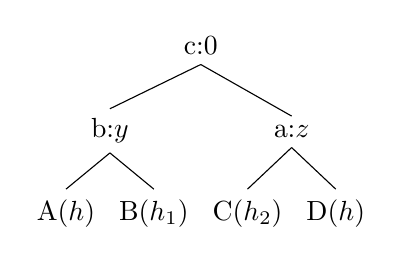
\begin{tikzpicture}
\Tree
    [.c:0
      [.b:$y$
        \edge[]; \node[very thick,rectangle]{A($h$)}; 
        \edge[]; \node[very thick,rectangle]{B($h_1$)};
      ]
      [.a:$z$
        \edge[]; \node[very thick,rectangle]{C($h_2$)};
        \edge[]; \node[very thick,rectangle]{D($h$)}; 
      ]
    ]       
\end{tikzpicture}
\end{center}
\caption{A general LR rotation. As before, the rectangles correspond
  to subtrees and the number in brackets to heights. The values of
  $h_1$ and $h_2$ can vary between two cases, $h_1=h$ and $h_2=h-1$ or
  $h_1=h-1$ and $h_2=h$ with $x=1$ or $x=-1$ respectively,
  corresponding, roughly, to the dashed and dotted cases consider
  before. {\bf A} is before, {\bf B} is after; as before the values of
  $y$ and $z$ depend on the value of $x$, if $x$ was one then $y=0$
  and $z=-1$, if $x$ was -1 then $y=1$ and $z=0$.
\label{fig_LR_complicated}}
\end{figure}




\begin{table}
\begin{lstlisting}[numbers=left]
struct node * rotate_lr(struct node * here)
{
  struct node * left=here->left;
  struct node * left_right=left->right;

  left->right=left_right->left;
  left_right->left=left;

  here->left=left_right->right;
  left_right->right=here;
		  
  if(left_right->balance==1)
    here->balance=-1;
  else
    here->balance=0;
  
  if(left_right->balance==-1)
    left->balance=1;
  else
    left->balance=0;
		  
  here=left_right;
  
  here->balance=0;
  
  return here;
}
\end{lstlisting}
\caption{The LR rotation. In lines 3 and 4 news pointer are made to
  keep track of {\bf here}$->$left and {\bf
    here}$->$left$->$right. The new balance factors at the end depend
  on the balance factor {\bf left\_right} had, just as the balance
  factors $y$ and $z$ depended on $x$.\label{c_LR}}
\end{table}

This leaves the issue of how the balance factors are updated. This is
done by a process of, in a sense, pushing the potential trouble upwards
until it either sorts itself out or becomes actual trouble and gets
fixed.  

Imagine adding a new node, called {\bf new} to the left of an existing
node, which we'll call {\bf here}. If the existing node has balance
factor one then adding {\bf new} would change it to two and a rotation
would be needed. Alternatively, the node might have a balance factor
of zero, in which case its new balance factor would be one and the
subtree coming from {\bf here} is now one longer than it used to be;
this needs to be addressed by considering what happens to {\bf here}'s
parent and so the process iterates with the balance factor of {\bf
  here}'s parent being looked at. Finally, {\bf here} might have had a
balance factor of -1, in which case its balance factor become zero
and, since the length of the substree rooted in {\bf here} has been
unchanged there is nothing more to do. Obviously, as far as iterating
this process is concerned {\bf new} can either be a new node, or a
subtree rooted in {\bf new} that is one longer than it used to be and
what applied to adding to the left also works for adding to the right,
except one is taken from the balance factor of {\bf here} instead of
one being added. The code that does this can be seen in Table~\ref{c_balance}.

\begin{table}
\begin{lstlisting}[numbers=left]
struct node * add_node_r(struct node * here,int new_entry,int * work_needed)
{
  if(here==NULL)
    {
      *work_needed = 1;
      return make_node(new_entry);
    }
  
  if(new_entry<here->entry)
    {
      here->left = add_node_r(here->left,new_entry,work_needed);
      if(*work_needed)
	{
	  switch(here->balance)
	    {
	    case -1:
	      here->balance=0;
	      *work_needed=0;
	      return here;
	    case 0:
	      here->balance=1;
	      return here;
	    case 1:
	      if(here->left->balance==1)
		here=rotate_ll(here);
	      else
		here=rotate_lr(here);
	      *work_needed=0;
	      return here;
	    }
	}
    }
  else
    {
      [RIGHT CASE]
  }
  return here;

}
\end{lstlisting}
\caption{Updating the balance factor. This recursive function uses an int called work\_needed to decide if an addition is resolved. It works down the tree until it finds where to add the new node, this happens at line 3-7, as it returns up the recursion it updates the balance factors if work\_needed is one, this uses the switch command from lines 14-30, if the balance factor is one then it should be changed to two and a rotation is done to avoid that, if it is zero it is changed to one and if it is -1 it is changed to zero and work needed is set to zero. The right version is similar and can be seen in the overall program {\tt AVL\_tree.c}.\label{c_balance}}
\end{table}


\end{document}
